\documentclass[tikz]{standalone}
\usetikzlibrary{patterns}
\usetikzlibrary{shapes,arrows}
\usetikzlibrary{decorations.pathreplacing, positioning}
\definecolor{greengreen}{rgb}{0.0, 0.42, 0.24}
\definecolor{calpolypomonagreen}{rgb}{0.12, 0.3, 0.17}
\definecolor{forestgreen}{rgb}{0.13, 0.55, 0.13}

\begin{document}
\noindent
  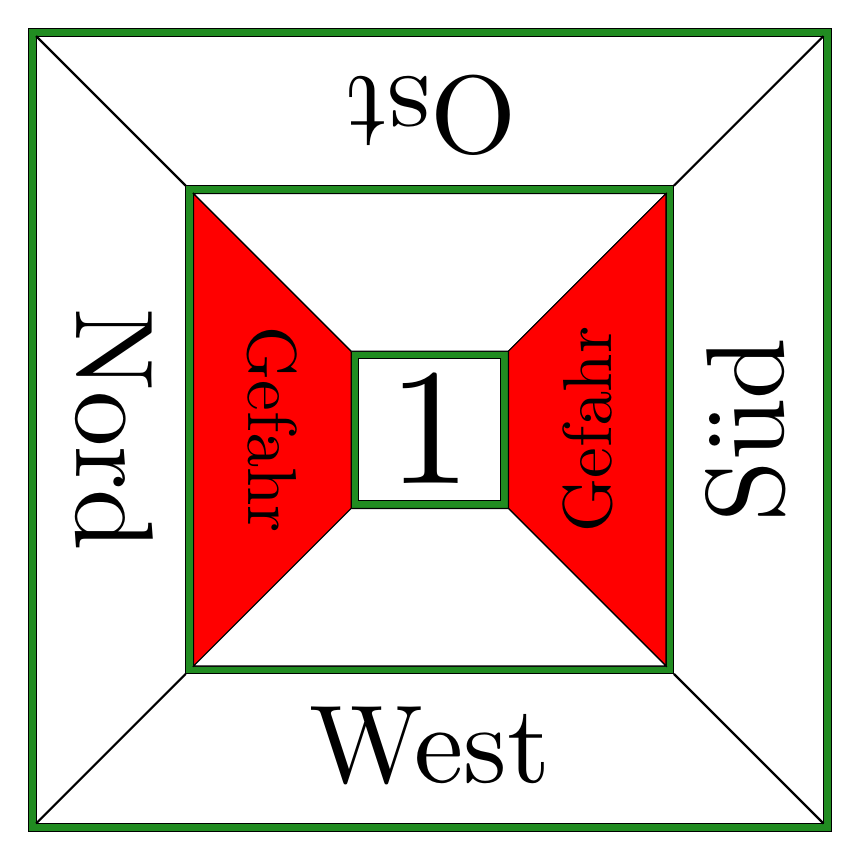
\begin{tikzpicture}

    \draw[fill=forestgreen] (-0.1,-0.1) -- (-0.1,10.1) -- (10.1, 10.1) -- (10.1, -0.1) -- cycle;
    \draw[fill=white] (0,0) -- (0,10) -- (10, 10) -- (10, 0) -- cycle;
    \draw[fill=forestgreen] (1.9, 1.9) -- (8.1,1.9) -- (8.1, 8.1) -- (1.9, 8.1) -- cycle;
    \draw[fill=white] (2, 2) -- (8,2) -- (8,8) -- (2,8) -- cycle;
    \draw[fill=forestgreen] (4, 4) -- (4,6) -- (6, 6) -- (6, 4) -- cycle;
    \draw[fill=white] (4.1, 4.1) -- (4.1,5.9) -- (5.9, 5.9) -- (5.9, 4.1) -- cycle;




    \draw[fill=red] (2,2) -- (2,8) -- (4, 6) -- (4, 4) -- cycle;
    \draw[fill=white] (2,8) -- (8,8) -- (6, 6) -- (4, 6) -- cycle;
    \draw[fill=red] (8,8) -- (8,2) -- (6, 4) -- (6, 6) -- cycle;
    \draw[fill=white] (2,2) -- (4,4) -- (6, 4) -- (8, 2) -- cycle;

    \node[very thick, rotate=270, scale=2.5] at (3,5) {Gefahr};
    \node[very thick, rotate=180, scale=2.5] at (5,7) {};
    \node[very thick, rotate=90, scale=2.5] at (7, 5) {Gefahr};
    \node[very thick, rotate=0, scale=2.5] at (5, 3) {};

    \node[very thick, rotate=270, scale=4] at (1,5) {Nord};
    \node[very thick, rotate=180, scale=4] at (5,9) {Ost};
    \node[very thick, rotate=90, scale=4] at (9, 5) {Süd};
    \node[very thick, rotate=0, scale=4] at (5, 1) {West};

    \draw[thick] (0,0) -- (1.9,1.9);
    \draw[thick] (0,10) -- (1.9,8.1);
    \draw[thick] (10,10) -- (8.1,8.1);
    \draw[thick] (10,0) -- (8.1,1.9);


    \node[very thick, rotate=0, scale=6] at (5, 5) {1};

  \end{tikzpicture}%
\end{document}
